\section{曲空间中的径向运动}
\label{sec:phys-ghs-geometric-radial}

平直空间中的离心项同时记录角向谱和径向体积测度。若空间有曲率，球壳面积不再按 $r^{d-1}$ 增长，前面的测度变换仍然适用，但会产生新的势项。先确定这些项，才能判断曲率怎样移动阈值和改变径向谱。

设空间维数为 $d=m+1$，度规和体积元为
\[
g=\dd r^2+a(r)^2h,\qquad
\dd\mu_g=a(r)^m\dd r\,\dd\mu_h,
\]
其中 $h$ 是紧致无边界截面 $\Sigma$ 上的无量纲黎曼度规，$a(r)>0$ 有长度量纲。取正交角模态 $-\Delta_hY_j=\lambda_jY_j$，$\lambda_j$ 无量纲。质量为 $\mu$ 的标量粒子在实径向势 $V(r)$ 中的哈密顿量为
\[
H=-\frac{\hbar^2}{2\mu}\Delta_g+V(r).
\]
这里选择拉普拉斯动力学；若物理模型另外含有曲率耦合，它是另一个必须指定的乘法势，不能从坐标变换自动推出。

\begin{proposition}[含测度的酉径向约化]
\label{prop:phys-ghs-warped-radial}
在角模态 $Y_j$ 上，令 $\psi=f_j(r)Y_j$，$u_j=a^{m/2}f_j$。则径向范数变为 $\int|u_j|^2\dd r$，相应哈密顿量是
\begin{equation}
H_j=-\frac{\hbar^2}{2\mu}\frac{\dd^2}{\dd r^2}+V_{j,\mathrm{eff}}(r),
\quad
V_{j,\mathrm{eff}}=V+\frac{\hbar^2}{2\mu}
\left[\frac{\lambda_j}{a^2}+\frac m2\frac{a''}{a}
+\frac{m(m-2)}4\left(\frac{a'}a\right)^2\right].
\label{eq:phys-ghs-warped-potential}
\end{equation}
此酉等价同时要求将原算子的自伴定义域映到新空间。
\end{proposition}
\begin{proof}
由散度形式，
\[
\Delta_g(f_jY_j)=\left[f_j''+m\frac{a'}a f_j'
-\frac{\lambda_j}{a^2}f_j\right]Y_j.
\]
令 $b=m/2$，$f_j=a^{-b}u_j$，逐次微分得到
\begin{align*}
f_j'&=a^{-b}\left(u_j'-b\frac{a'}a u_j\right),\\
f_j''&=a^{-b}\left[u_j''-2b\frac{a'}a u_j'
+\left(b(b+1)\frac{(a')^2}{a^2}-b\frac{a''}a\right)u_j\right].
\end{align*}
代回径向表达式，$u_j'$ 的系数为 $2b-m=0$；$u_j$ 的系数为
\[
\frac{\lambda_j}{a^2}+b\frac{a''}a
+b(m-b-1)\frac{(a')^2}{a^2},
\]
即所述有效势。又有 $\int|f_j|^2a^m\dd r=\int|u_j|^2\dd r$，因而变换等距且满射。对原定义域中的所有函数施加同一变换，才把形式微分恒等式提升为算子等价。
\end{proof}

若原端点的坐标导数条件是 $f_j'=\gamma f_j$，新条件是 $u_j'=[\gamma+(m/2)a'/a]u_j$。因此只改势而照搬边界参数会定义另一个量子模型。若 $a$ 在端点趋零，需用前面的极限点、极限圆判据和完整空间的正则条件选择定义域。

\begin{example}[三维常曲率空间的谱阈值]
\label{ex:phys-ghs-curvature-threshold}
取 $m=2$、单位二球截面，$\lambda_\ell=\ell(\ell+1)$，并令 $V=0$。曲率长度为 $L$，平直空间、三球和双曲空间分别对应
\[
a_0=r,\quad a_+=L\sin(r/L),\quad a_-=L\sinh(r/L).
\]
它们的径向区间分别为 $(0,\infty)$、$(0,\pi L)$、$(0,\infty)$。将尺度函数代入 \cref{eq:phys-ghs-warped-potential}，得到
\begin{align*}
V_{\ell,0}&=\frac{\hbar^2}{2\mu}\frac{\ell(\ell+1)}{r^2},\\
V_{\ell,+}&=\frac{\hbar^2}{2\mu L^2}
\left[\frac{\ell(\ell+1)}{\sin^2(r/L)}-1\right],\\
V_{\ell,-}&=\frac{\hbar^2}{2\mu L^2}
\left[\frac{\ell(\ell+1)}{\sinh^2(r/L)}+1\right].
\end{align*}
三球的 $s$ 波取 $u=\sin(r/L)$，两端正则且 $H_0u=0$，对应常数原始波函数；负的几何势并没有产生负的拉普拉斯本征值。双曲空间的 $s$ 波则在远处留下阈值 $E_{\mathrm{th}}=\hbar^2/(2\mu L^2)$，常数原始波函数不可归一化。

三球的全部正则径向解写为
\[
u_{n\ell}=\sin^{\ell+1}x\,C_{n-\ell}^{(\ell+1)}(\cos x),
\quad x=r/L,\quad n\ge\ell.
\]
置 $z=\cos x$ 代入径向方程，得到
\[
(1-z^2)F''-(2\ell+3)zF'
+(n-\ell)(n+\ell+2)F=0,
\]
故 $E_n=\hbar^2n(n+2)/(2\mu L^2)$。对固定 $n$ 求和磁简并度，$\sum_{\ell=0}^n(2\ell+1)=(n+1)^2$。球面的两端正则条件和角向表示共同决定这一离散谱。
\end{example}

\begin{figure}[htbp]
\centering
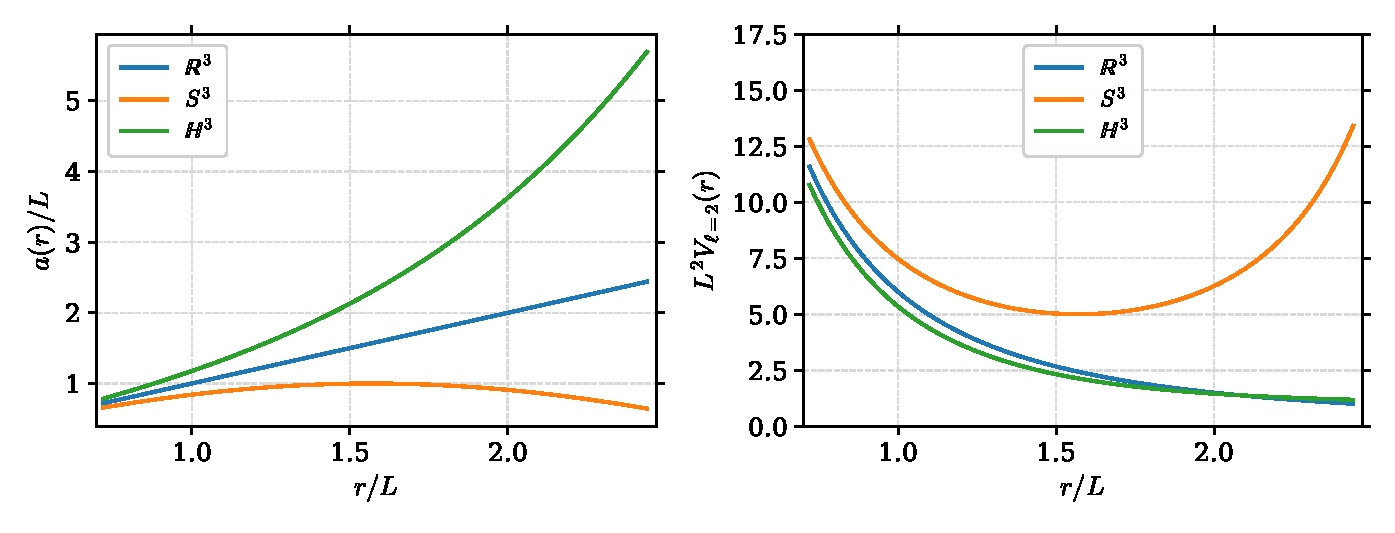
\includegraphics[width=.86\linewidth]{content/AdvancedPhysics/figures/geometry-highspin/warped_radial_potentials.pdf}
\caption{三维常曲率空间的尺度函数与径向势。图中长度以 $L$ 为单位，势以 $\hbar^2/(2\mu L^2)$ 为单位，取 $\ell=2$。靠近原点的主导离心奇性相同；三球第二极点的边界条件仍须另行施加。}
\label{fig:phys-ghs-warped-potential}
\end{figure}

\cref{fig:phys-ghs-warped-potential} 中的曲率位移来源于径向测度的酉变换。回到一般截面，只需替换角向本征值；若曲率势还依赖角坐标，则不同角模态会耦合，不能继续使用独立的一维方程。
